\documentclass[a4paper,12pt]{article}
\usepackage{float}
\usepackage{amsmath, amssymb}
\usepackage{graphicx}
\usepackage{multirow}
\usepackage{booktabs}
\usepackage{geometry}
\usepackage{enumitem}
\usepackage{listings}
\usepackage{xcolor}
\usepackage{tikz}
\geometry{margin=1in}
\setlength{\parindent}{0pt}

\usepackage[numbers]{natbib}
\usepackage{multicol}
\usepackage[bookmarks=true]{hyperref}
\usepackage[font=footnotesize]{subfig}
\usepackage{mathtools}
\usepackage[labelfont=bf]{caption}
\usepackage{wrapfig}
\usepackage[ruled,vlined]{algorithm2e}

\begin{document}

\begin{center}
    \Large \textbf{Assignment 4} \\[6pt]
    \today
\end{center}

% ------------------------------------------------------------
\section*{A. Bayes}

We are given a binary random variable describing the state of a door:
\[
open \in \{open, \neg open\}.
\]

The sensor observation is \( z = 42 \), with the following conditional probabilities:
\[
P(z=42 \mid open) = \frac{2}{3}, \quad
P(z=42 \mid \neg open) = \frac{1}{3}.
\]

The prior probability of the door being open is:
\[
P(open) = \frac{3}{5},
\]
which implies:
\[
P(\neg open) = 1 - P(open) = \frac{2}{5}.
\]

Using Bayes' theorem, the posterior probability of the door being open given the observation \( z=42 \) is:
\[
P(open \mid z=42) =
\frac{P(z=42 \mid open)\,P(open)}{P(z=42)}.
\]

The marginal likelihood \( P(z=42) \) is computed using the law of total probability:
\[
\begin{aligned}
P(z=42) &=
P(z=42 \mid open)\,P(open)
+ P(z=42 \mid \neg open)\,P(\neg open) \\
&=
\frac{2}{3}\cdot\frac{3}{5}
+ \frac{1}{3}\cdot\frac{2}{5} \\
&=
\frac{2}{5} + \frac{2}{15}
= \frac{8}{15}.
\end{aligned}
\]

Substituting into Bayes' formula yields:
\[
\begin{aligned}
P(open \mid z=42)
&=
\frac{\frac{2}{3}\cdot\frac{3}{5}}{\frac{8}{15}}
= \frac{\frac{2}{5}}{\frac{8}{15}}
= \frac{2}{5}\cdot\frac{15}{8}
= \frac{3}{4}.
\end{aligned}
\]

\paragraph{Final Result:}
\[
\boxed{P(open \mid z=42) = 0.75}
\]

Thus, given the sensor observation \( z = 42 \), the probability that the door is open is \(75\%\).



% ------------------------------------------------------------
\section*{B. Mapping with Raw Odometry}
Screenshots of the map-building process were taken at approximately $t \approx 2\,\text{s}$, $t \approx 8\,\text{s}$, and $t \approx 20\,\text{s}$.

\begin{figure}[H]
    \centering
    \setlength{\tabcolsep}{6pt}
    \begin{tabular}{ccc}
        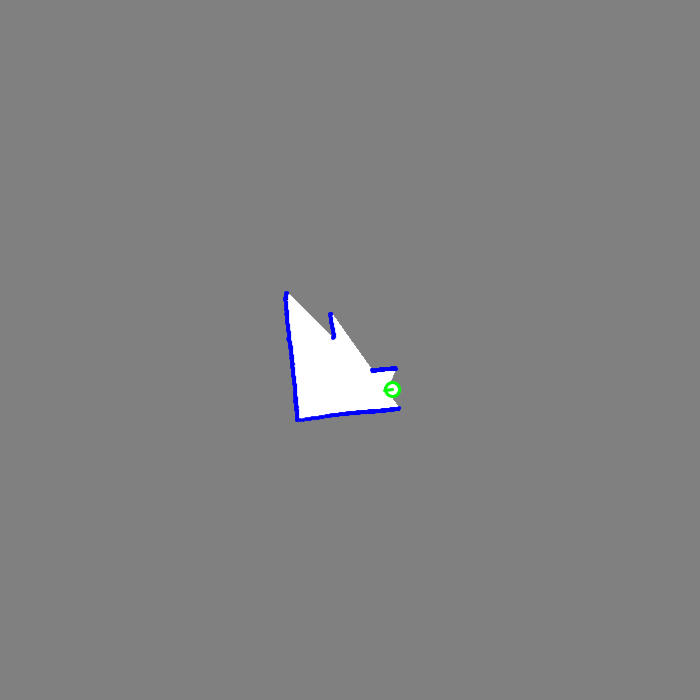
\includegraphics[width=0.3\textwidth]{imgs/odo_map_t1.png} &
        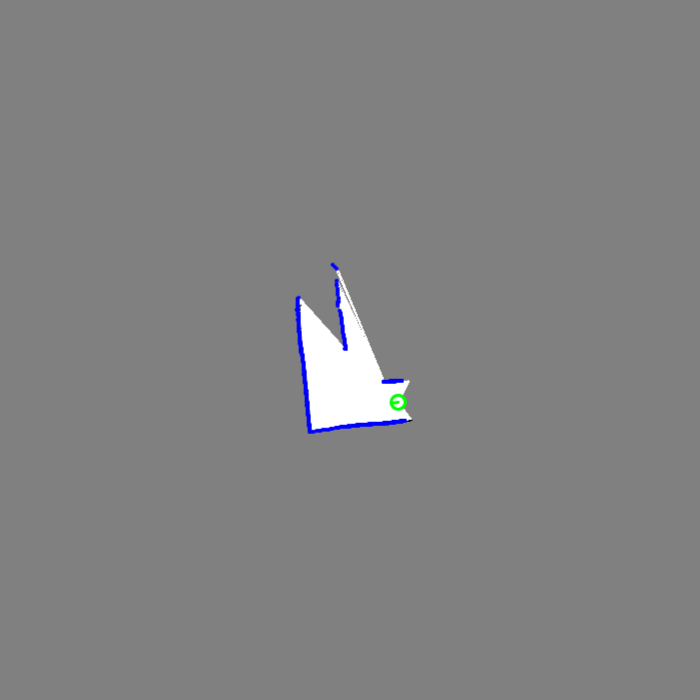
\includegraphics[width=0.3\textwidth]{imgs/odo_map_t2.png} &
        
\includegraphics[width=0.3\textwidth]{imgs/odo_map_t3.png} \\
        \small t$_1 \approx 2\,\text{s}$ &
        \small t$_2 \approx 8\,\text{s}$ &
        \small t$_3 \approx 20\,\text{s}$
    \end{tabular}
    \caption{Occupancy grid maps generated using raw odometry at three different time steps.}
    \label{fig:odometry_mapping}
\end{figure}

At early stages of the mapping process ($t_1$ and $t_2$), the generated map appears relatively accurate. As time progresses, accumulated errors lead to an increasingly distorted map, which becomes clearly visible at $t_3$. This behavior can primarily be attributed to unmodeled odometry drift and sensor noise, which are not explicitly accounted for in the simplified update scheme.

Furthermore, the Simple Counting Method treats all laser hits and misses as equally reliable, regardless of measurement uncertainty or distance-related noise. In practice, real sensors exhibit varying confidence levels depending on environmental and measurement conditions.  A probabilistic occupancy update that assigns weighted contributions to sensor measurements would therefore be expected to improve mapping accuracy.

\section*{C. Monte Carlo Localization: Particle Filter}

\subsection*{Likelihood Field}
\begin{figure}[H]
    \centering
    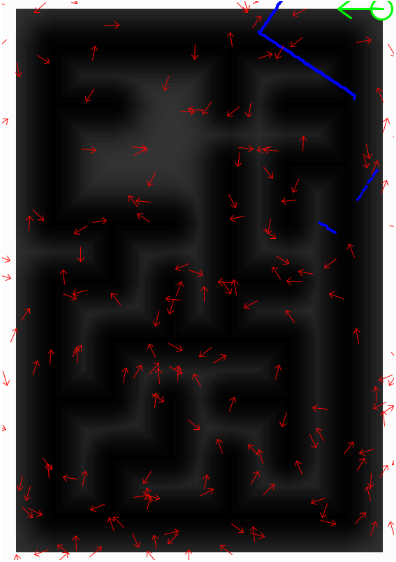
\includegraphics[width=0.35\textwidth]{imgs/likelihood_field.png}
    \caption{Visualization of the likelihood field.}
\end{figure}

\subsection*{Uniformly Distributed Particle Set Map}
Starting from a uniform particle distribution, the filter converges to the correct robot pose over time. Screenshots were taken at $t = 5\,\text{s}$, $10\,\text{s}$, $14\,\text{s}$, $20\,\text{s}$, $30\,\text{s}$, $42\,\text{s}$, $60\,\text{s}$, and $75\,\text{s}$.

\begin{figure}[H]
    \centering
    \setlength{\tabcolsep}{2pt}
    \begin{tabular}{cccc}
        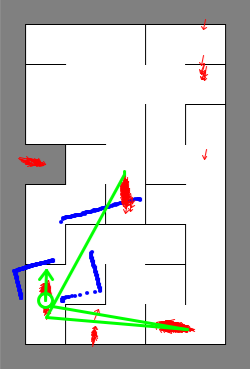
\includegraphics[width=0.17\textwidth]{imgs/combined_unidist_loc_t1.png} &
        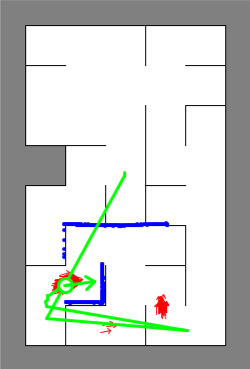
\includegraphics[width=0.17\textwidth]{imgs/combined_unidist_loc_t2.png} &
        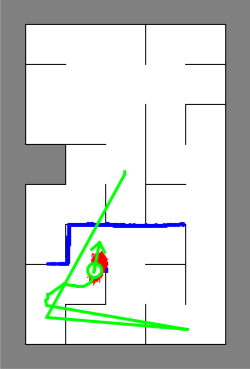
\includegraphics[width=0.17\textwidth]{imgs/combined_unidist_loc_t3.png} &
        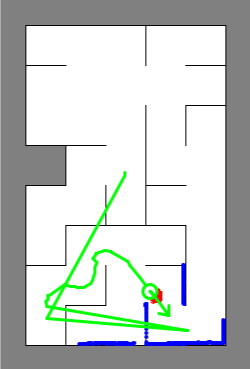
\includegraphics[width=0.17\textwidth]{imgs/combined_unidist_loc_t4.png} \\
        \small $t_1 \approx 5\text{s}$ & \small $t_2 \approx 10\text{s}$ & \small $t_3 \approx 14\text{s}$ & \small $t_4 \approx 20\text{s}$ \\
        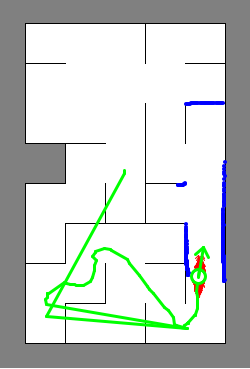
\includegraphics[width=0.17\textwidth]{imgs/combined_unidist_loc_t5.png} &
        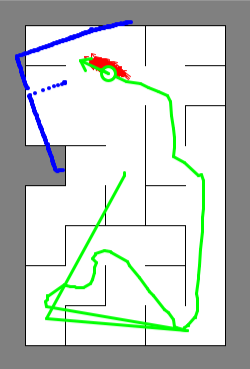
\includegraphics[width=0.17\textwidth]{imgs/combined_unidist_loc_t6.png} &
        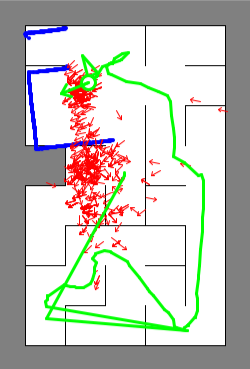
\includegraphics[width=0.17\textwidth]{imgs/combined_unidist_loc_t7.png} &
        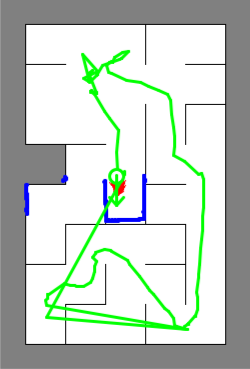
\includegraphics[width=0.17\textwidth]{imgs/combined_unidist_loc_t8.png} \\
        \small $t_5 \approx 30\text{s}$ & \small $t_6 \approx 42\text{s}$ & \small $t_7 \approx 60\text{s}$ & \small $t_8 \approx 75\text{s}$
    \end{tabular}
    \caption{Global localization using a uniformly initialized particle set at the required time steps.}
    \label{fig:uniform_localization_times}
\end{figure}

\subsection*{Gaussian Distributed Particle Map}
In contrast to global localization, the particle filter is initialized using a Gaussian distribution.
\begin{figure}[H]
    \centering
    \setlength{\tabcolsep}{2pt}
    \begin{tabular}{cccc}
        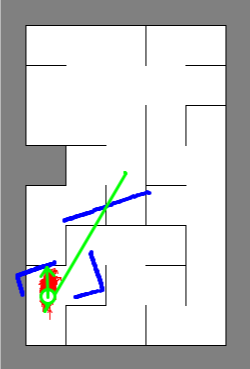
\includegraphics[width=0.17\textwidth]{imgs/gauss_dist_loc_t1.png} &
        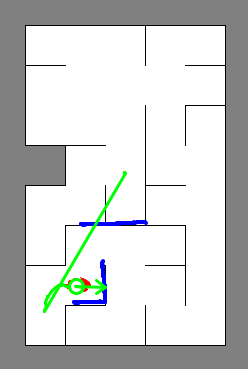
\includegraphics[width=0.17\textwidth]{imgs/gauss_dist_loc_t2.png} &
        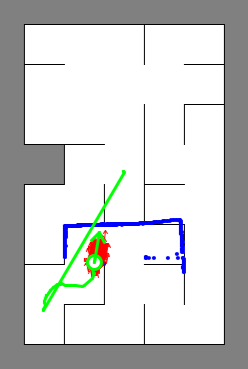
\includegraphics[width=0.17\textwidth]{imgs/gauss_dist_loc_t3.png} &
        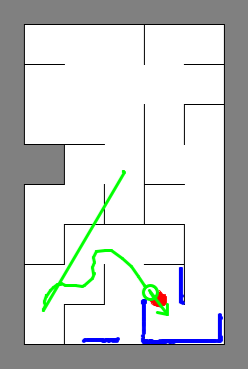
\includegraphics[width=0.17\textwidth]{imgs/gauss_dist_loc_t4.png} \\
        \small $t_1 \approx 5\text{s}$ & \small $t_2 \approx 10\text{s}$ & \small $t_3 \approx 14\text{s}$ & \small $t_4 \approx 20\text{s}$ \\
        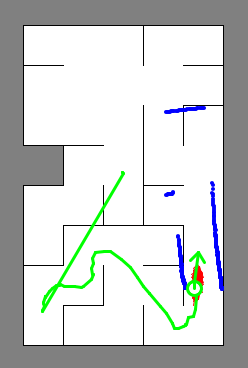
\includegraphics[width=0.17\textwidth]{imgs/gauss_dist_loc_t5.png} &
        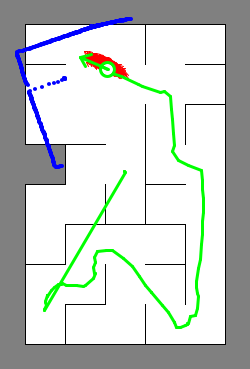
\includegraphics[width=0.17\textwidth]{imgs/gauss_dist_loc_t6.png} &
        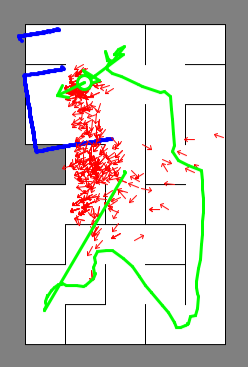
\includegraphics[width=0.17\textwidth]{imgs/gauss_dist_loc_t7.png} &
        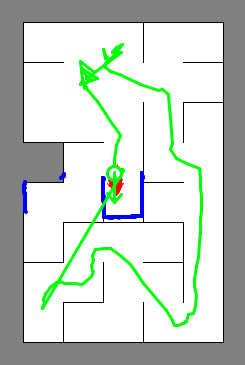
\includegraphics[width=0.17\textwidth]{imgs/gauss_dist_loc_t8.png} \\
        \small $t_5 \approx 30\text{s}$ & \small $t_6 \approx 42\text{s}$ & \small $t_7 \approx 60\text{s}$ & \small $t_8 \approx 75\text{s}$
    \end{tabular}
    \caption{Tracking using a Gaussian-initialized particle set at the required time steps.}
    \label{fig:gaussian_localization_times}
\end{figure}





\end{document}
